
%(BEGIN_QUESTION)
% Copyright 2006, Tony R. Kuphaldt, released under the Creative Commons Attribution License (v 1.0)
% This means you may do almost anything with this work of mine, so long as you give me proper credit

Many industrial pressure sensing elements, especially diaphragms and bellows, are equipped with {\it stops} to limit the physical travel of the sensing element:

$$\includegraphics[width=15.5cm]{i00224x01.eps}$$

$$\includegraphics[width=15.5cm]{i00224x02.eps}$$

What important purpose is served by a {\it stop} in a pressure measuring instrument?

\underbar{file i00224}
%(END_QUESTION)





%(BEGIN_ANSWER)

A {\it stop} prevents the pressure element from being excessively strained by overpressure.  Ultimately, it helps to prevent rupture of the element in the case of accidental overpressure.

When a pressure element flexes so far that it comes to rest against a stop, the stop begins to provide the opposition force to the force generated by the applied pressure, so the element does not have to strain further.  Ideally, the stop(s) in an instrument will be set up to limit the element's travel enough so that its elastic limit is never exceeded.  However, the presence of a stop does not guarantee that the instrument will remain within calibration specifications after exposure to an overpressure!

Stops are important even in force-balance transmitters where the pressure element (hypothetically) never moves.  Under certain overpressure conditions, the element will generate more force than the balance mechanism is able to counter, and so the pressure element will most definitely strain.  A stop in a force-balance instrument helps ensure that even if the element strains, it will not strain too much.

%(END_ANSWER)





%(BEGIN_NOTES)


%INDEX% Measurement, pressure: overpressure ``stops''

%(END_NOTES)


